%!TEX root = ../dokumentation.tex


\chapter{Validierung des Systems}\label{chap:validierung}

Nachdem das Aufnehmen und Darstellen von Räumen funktioniert, wird die Genauigkeit des Systems untersucht. Zudem werden Versuche zu verschiedenen Auflösungen und unterschiedlicher Sensoren durchgeführt.  


\section{Genauigkeit des Systems}

Um die Genauigkeit des Systems zu überprüfen, wird ein Raum mit dem Lidar-System vermessen. Zudem wird der Raum händisch vermessen und der Grundriss mit der Software ''Sweet Home 3D'' erstellt. Anschließend wird die 3D-Darstellung mit dem Grundriss des Raumes und weiterer markanter Gegenstände verglichen.
Bei dem Raum handelt es sich um einen Flur mit vielen Ecken, Türen und Gegenständen. Dadurch erhält man viele verschiedene Maße, die überprüft werden können. Der Grundriss des Raumes ist in Abbildung \ref{grundriss} dargestellt. Alle weiteren Maße des Raumes können direkt in der Software abgerufen werden.

\begin{figure}[H]
	\centering
	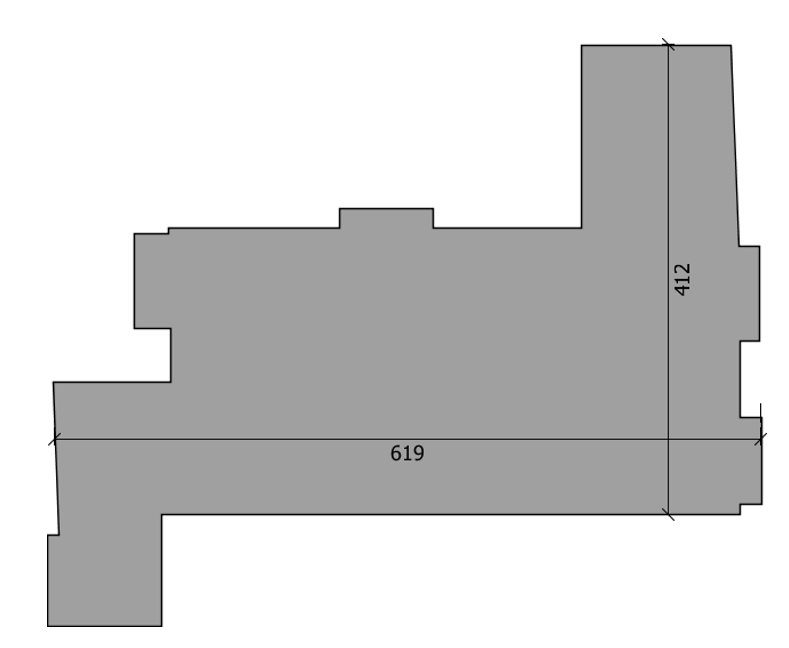
\includegraphics[width=0.6\textwidth]{images/Validierung/Grundriss}
	\caption{Grundriss des Testraums}
	\label{grundriss}
\end{figure}


Das Lidar-System wird im Raum aufgestellt. Die Position ist annähernd mittig und wird zudem bestimmt und in der Software eingetragen. Durch die Funktionsweise von Lidar Sensoren entstehen Schatten. So können beispielsweise Konturen hinter einer Wand, die die Lichtstrahlen reflektiert nicht detektiert werden. Diese Schatten werden ebenfalls im Grundriss eingezeichnet, um den Vergleich besser durchführen zu können. Die weißen Stellen innerhalb des Grundrisses in Abbildung \ref{grundrssmitschatte} stellen diese Schatten dar.

\begin{figure}[H]
	\centering
	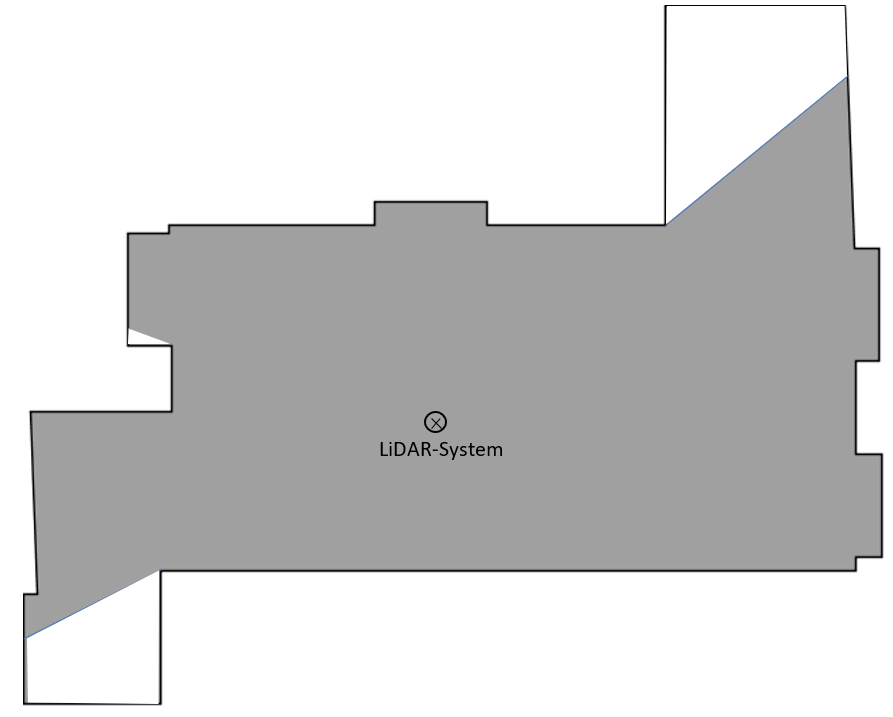
\includegraphics[width=0.7\textwidth]{images/Validierung/MitSchatten}
	\caption{Grundriss des Testraums}
	\label{grundrssmitschatte}
\end{figure}


Zum Vergleich wird nun der Grundriss benötigt, den das Lidar-System erstellt hat. Dazu wird die 3D Darstellung nur in z-Richtung betrachtet. Man erhält die Vogelperspektive des Raumes, bei dem der Grundriss auszumachen ist. 

\begin{figure}[H]
	\centering
	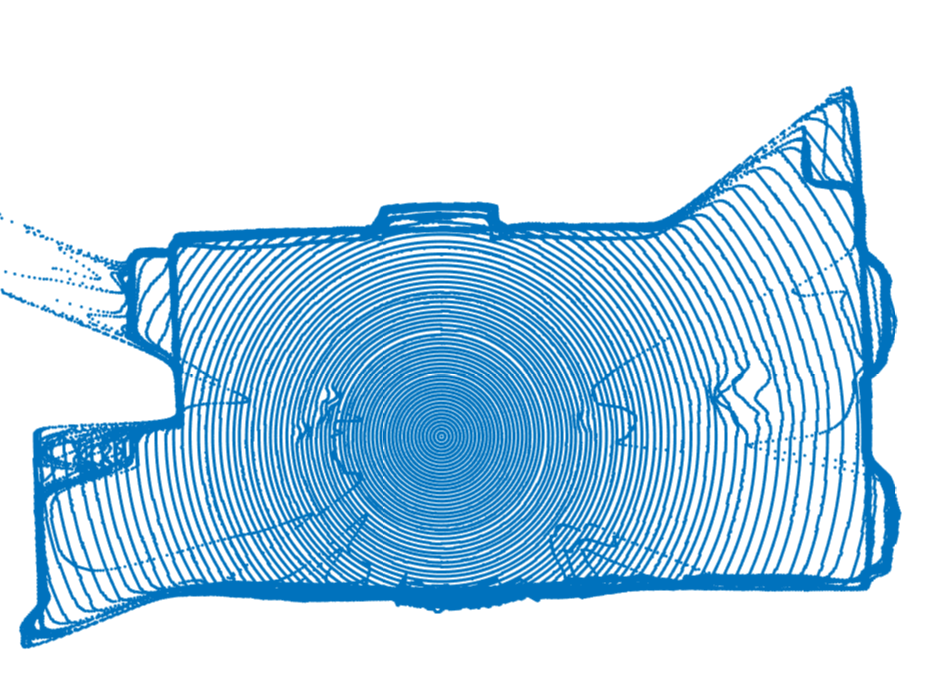
\includegraphics[width=0.7\textwidth]{images/Validierung/Vogelperspektive}
	\caption{Vogelperspektive des Testraums}
	\label{vogelperspektive}
\end{figure}


Zum grafischen Vergleich werden manuell erstellter Grundriss und die Vogelperspektive des Testraums mit einem Bildbearbeitungsprogramm im gleichen Maßstab übereinander gelegt.

\begin{figure}[H]
	\centering
	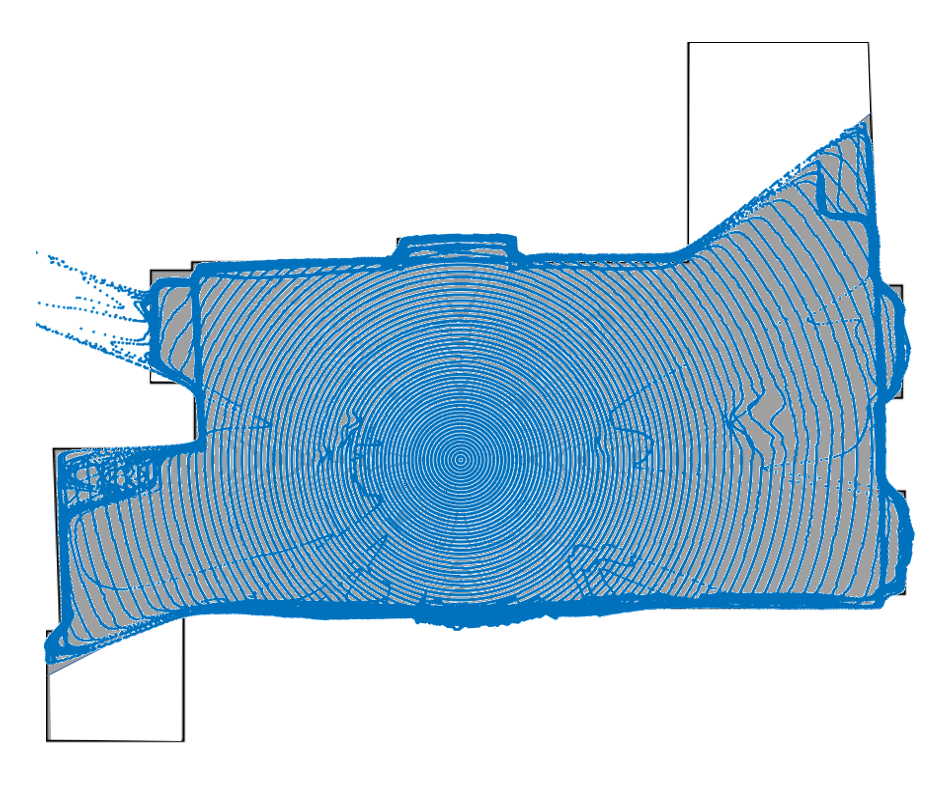
\includegraphics[width=0.7\textwidth]{images/Validierung/uebereinander}
	\caption{Grafischer Vergleich der Grundrisse}
	\label{uebereinander}
\end{figure}


Es ist zu erkennen, dass die beiden Grundrisse fast überall Übereinstimmen. Auffällig sind die vielen Messwerte, die auf der linken Seite außerhalb des Raums liegen. An dieser Stelle befindet sich eine Glastüre. Diese wird von einem Lidar-Sensor nicht detektiert, weswegen an dieser Stelle die Punkte abweichen. Zudem sind die Türrahmen auf der linken Seite nicht perfekt eckig, was auf weitere Schatten des Lasers schließen lässt.

Im 3D-Modell sind im Gegensatz zu dem Grundriss noch Möbel (links und rechts oben) zu erkenne. Zudem führen Lampen zu Unregelmäßigkeiten an der Decke.


\begin{figure}[H]
	\centering
	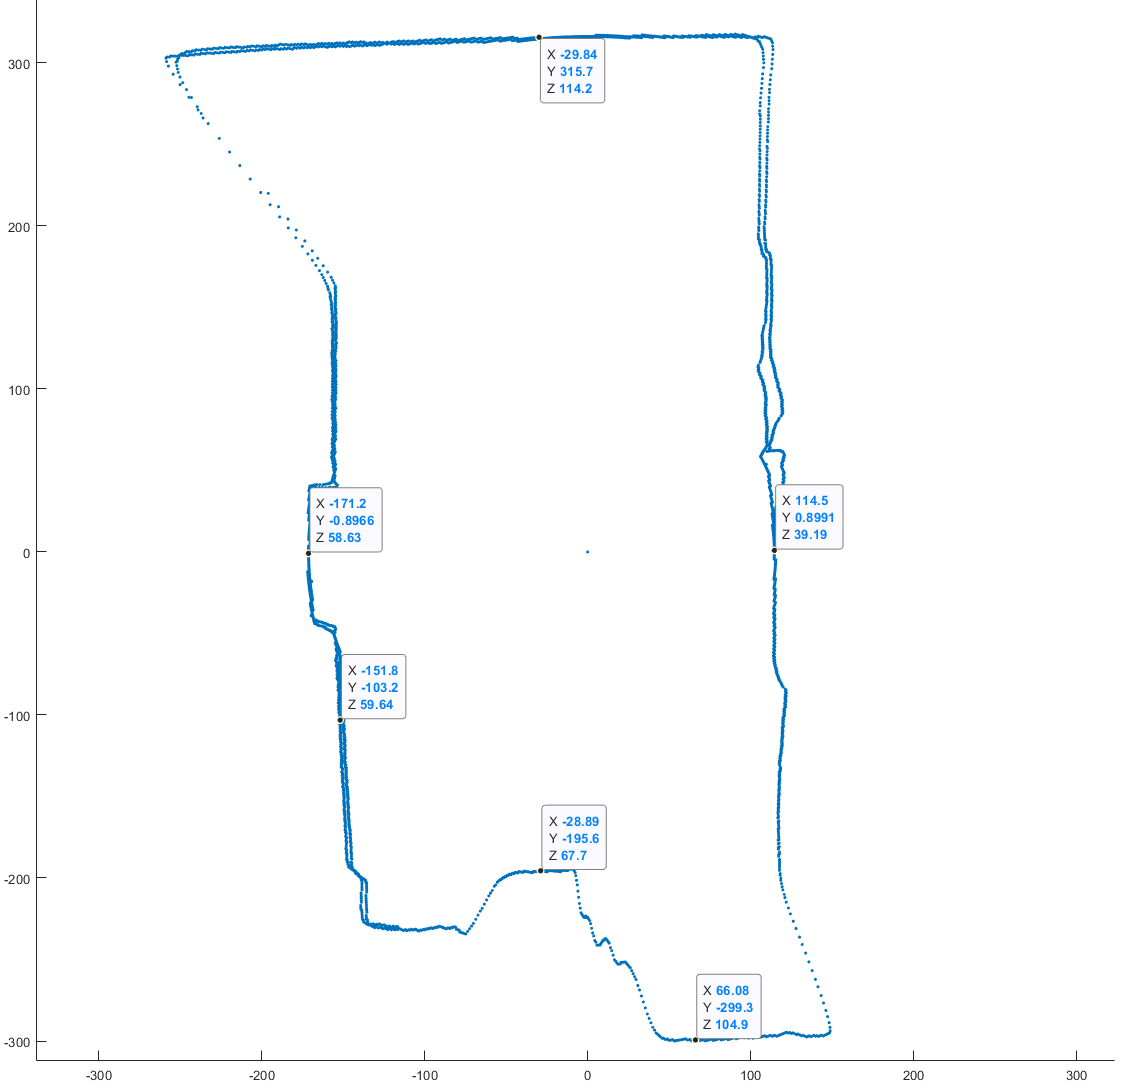
\includegraphics[width=0.7\textwidth]{images/Validierung/Genauigkeit/Messwerte.png}
	\caption{Messwerte über Data Coursor}
	\label{uebereinanawsdfder}
\end{figure}


\begin{figure}[htb]
	\centering
	\begin{minipage}[t]{0.45\linewidth}
		\centering
		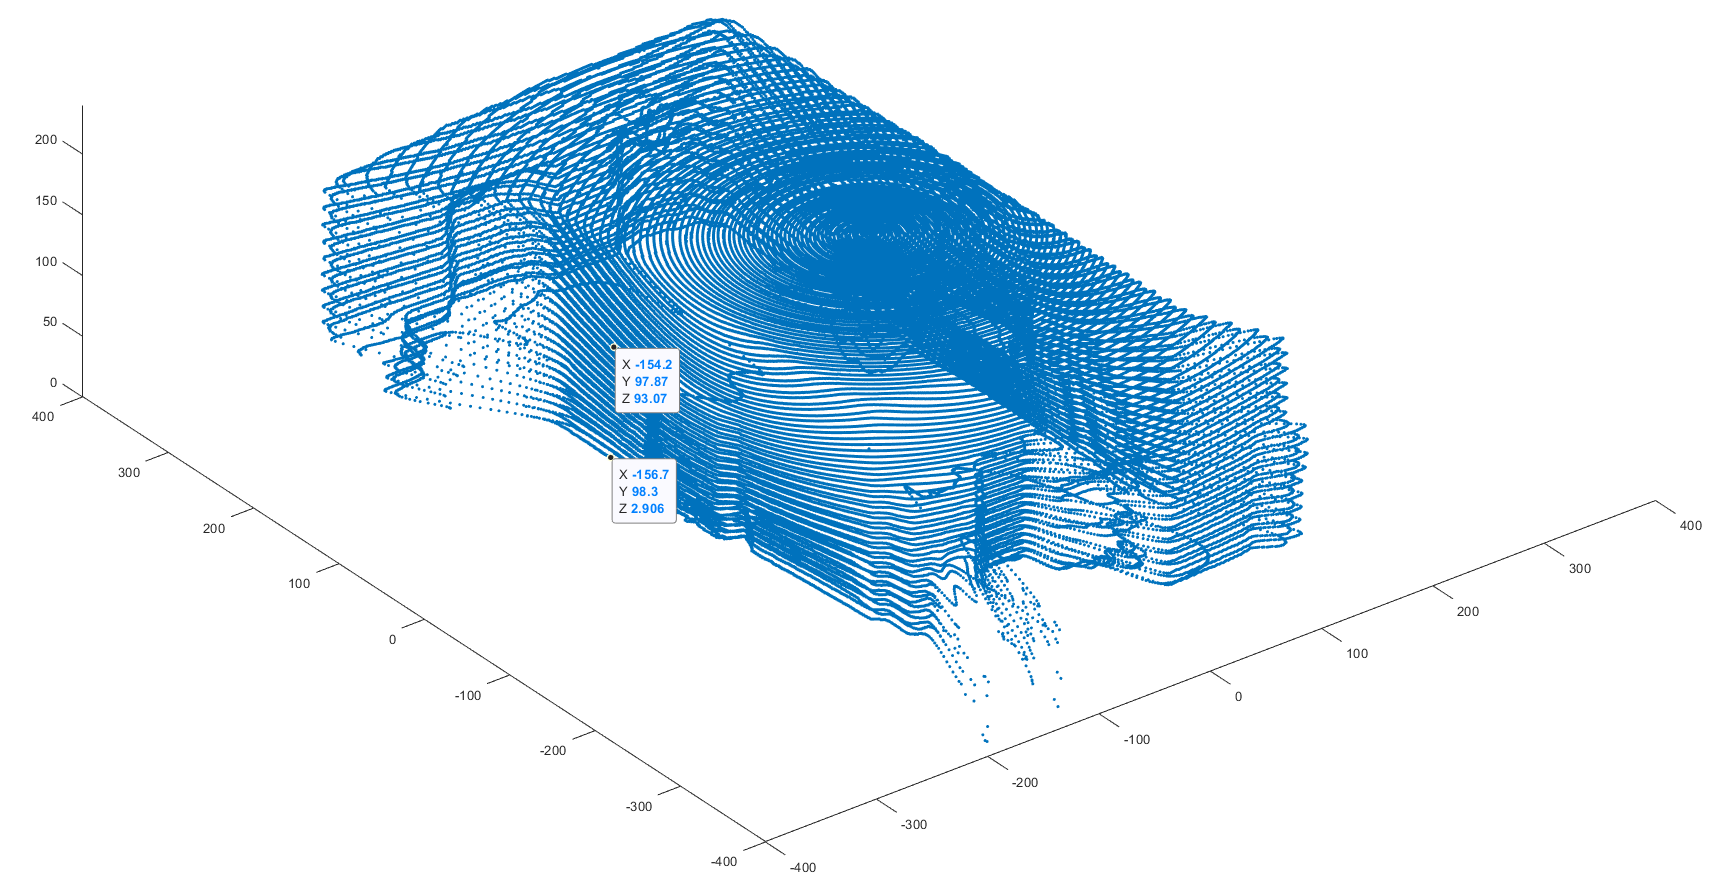
\includegraphics[width=1.2\linewidth]{images/Validierung/Genauigkeit/wandbreite_alles.png}
		\caption{Vogelperspektive niedrige Auflösung}
		\label{wandbreite_alles}
	\end{minipage}
	\hfill
	\begin{minipage}[t]{0.45\linewidth}
		\centering
		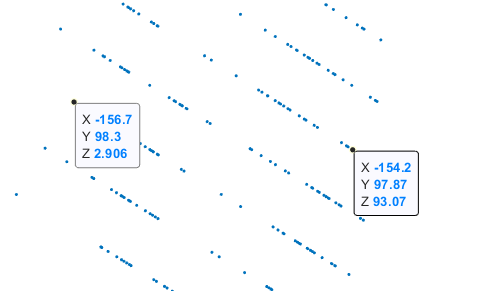
\includegraphics[width=1.2\linewidth]{images/Validierung/Genauigkeit/wandbreite.png}
		\caption{Vogelperspektive hohe Auflösung}
		\label{wandbreite_label}
	\end{minipage}
\end{figure}


\begin{figure}[H]
	\centering
	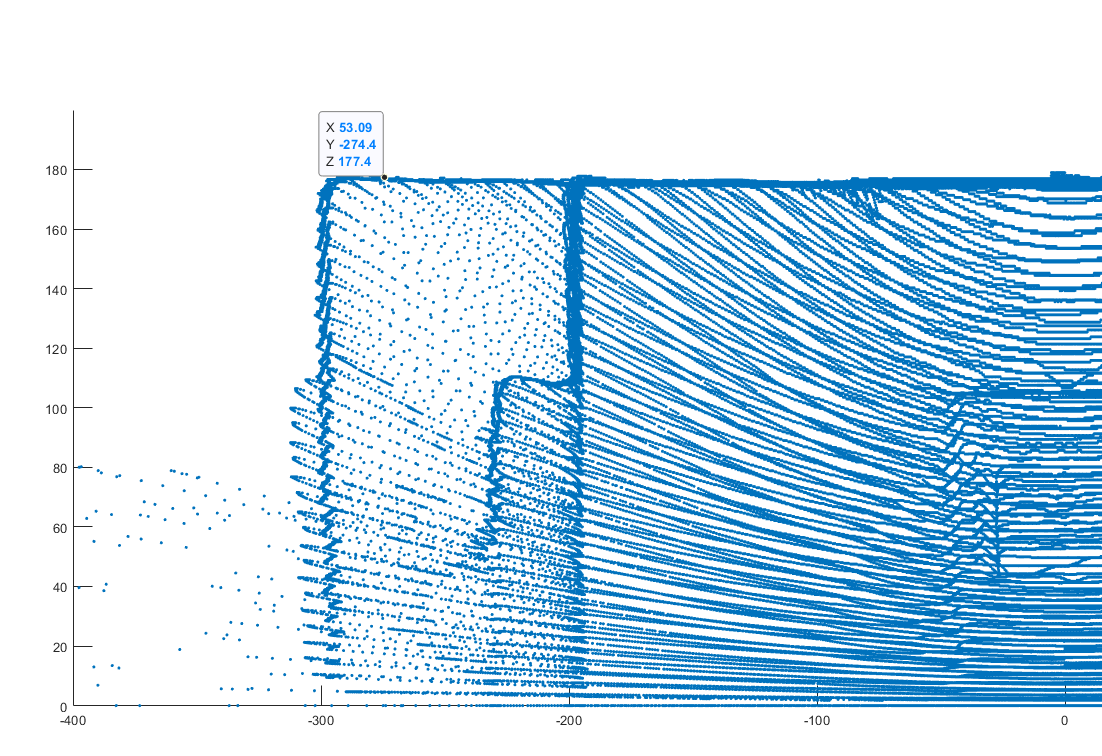
\includegraphics[width=0.7\textwidth]{images/Validierung/Genauigkeit/Hoehe}
	\caption{Grafischer Vergleich der Grundrisse}
	\label{uebereinaasdasfnder}
\end{figure}



\todo{Auswertung beschreiben, was kann man sehen?}
\todo{Linien an Seite raus weil Glas}
\todo{Höhe wird überprüft, Schrank, Bild usw, Messen mit Cursor}



\section{Vergleich verschiedener Auflösungen}

Durch das Einstellen verschiedener Schrittweiten der Schrittmotoren können unterschiedliche Auflösungen und Punkteverteilungen eingestellt werden. Derselbe Raum wird unter den gleichen Randbedingungen mit drei unterschiedlichen Einstellungen vermessen. Dabei bleibt sowohl die Position des Lidar-Sensors als auch der Sensor selbst gleich. Verändert wird sowohl die horizontale- als auch die vertikale Schrittweite. Dies kann im Code durch das Ändern weniger Parameter realisiert werden.

Bei den verschiedenen Auflösungen werden vor allem das Ergebnis und die benötigte Zeit zum Aufnehmen der Messdaten verglichen. Zudem soll dadurch eine Einstellung gefunden werden, die einen guten Kompromiss zwischen Auflösung und benötigter Zeit darstellt. 

Als Sensor wird der ''TF Mini Lidar'' verwendet.


\subsection{Übersicht über die Dauer, Auflösung und Anzahl an Messpunkten}

Die horizontale Auflösung wird im Code in achtel Schritten des Schrittmotors angegeben. Der Motor läuft im Achtelschrittbetrieb. Für eine gesamte Umdrehung des Motors werden 200 Vollschritte benötigt. Zudem entspricht die Übersetzung von Schrittmotor zur drehbaren Basis des Lidar-Systems 1:6. Es werden also 9600 Achtelschritte benötigt, um die Basis einmal um 360 Grad zu drehen. Die Auflösung in Grad bezogen auf die Angabe im Code kann mit Formel \ref{horizontialeAuflösung} berechnet werden. 

\begin{equation}\formelentry{Berechnung horizontiale Auflösung}
d = \frac{360}{200 \cdot 8 \cdot 6} \cdot x
\label{horizontialeAuflösung}
\end{equation}
\begin{flalign*}
&x = \text{Anzahl Achtelschritte des Motors (in Software)} \left[^{\circ} \right]&\\
&d = \text{reale Drehung des Sensors in horizontaler Richtung}\left[^{\circ} \right]&\\
\end{flalign*}

Die vertikale Grundeinheit sind Viertelschritte. Um den Sensor um die maximalen 90 Grad drehen zu können, werden 50 Vollschritte benötigt. Der Sensor ist direkt mit der Welle des Motors verbunden, wodurch keine Konstante für eine Übersetzung benötigt wird.

\begin{equation}\formelentry{Berechnung vertikale Auflösung}
d = \frac{360}{50 \cdot 4} \cdot x
\label{vertikaleAuflösung}
\end{equation}
\begin{flalign*}
&x = \text{Anzahl Viertelschritte des Motors (in Software)} \left[^{\circ} \right]&\\
&d = \text{reale Drehung des Sensors in horizontaler Richtung}\left[^{\circ} \right]&\\
\end{flalign*}


Die Menge der Messpunkte lässt sich über die Anzahl der horizontalen Messpunkte multipliziert mit der Anzahl der vertikalen Reihen berechnen.

Die benötigte Zeit ist linear zu der Anzahl der Messpunkte.

\begin{table}
	\centering
	\caption{Übersicht verschiedene Auflösungen}	
		\begin{tabular} [H] {|c|c|c|c|}
		\hline
		\textbf{}										 &\textbf{Auflösung gering} & \textbf{Auflösung mittel}	& \textbf{Auflösung hoch} \\ \hline
		\begin{tabular}[x]{@{}c@{}}
			\textbf{Auflösung}\\\textbf{horizontial [$^{\circ} $]}
		\end{tabular}
			 & 1,2 	& 0,15 	 & 0,15			\\  \hline
		\begin{tabular}[x]{@{}c@{}}
			\textbf{Auflösung}\\\textbf{vertikal [$ ^{\circ} $]}
		\end{tabular}	 
			 & 14,4 & 7,2 	 & 3,6  		\\ \hline
		\begin{tabular}[x]{@{}c@{}}
			\textbf{Anzahl}\\\textbf{Messpunkte}
		\end{tabular}		 
			 & 7524 & 120049 & 240099 		\\ \hline
		\textbf{Dauer [min]}
			 & 2    & 31	 & 62 		 	\\ \hline
		
		\end {tabular}
		\label{uebersicht}
\end{table}


\subsection{Vergleich der unterschiedlichen Auflösungen}

Im Anschluss werden die 3D-Darstellungen grafisch verglichen und beurteilt.Vor allem die Darstellung von Details und die Richtigkeit der Maße wird überprüft. 

Um den Vergleich zu erleichtern, werden Bilder aus der jeweils gleichen Perspektive erstellt und verglichen. Der Maßstab ist bei jeder Darstellung identisch.
 
Die Aufnahme mit niedriger Auflösung besteht aus rund 7500 Bildpunkten. Die horizontale Auflösung ist mit 1,2 Grad Abstand zwischen zwei Punkten für nicht weit entfernte Gegenstände ausreichend. Bei größerer Entfernung wie z.B. in den Ecken des Raumes wird diese Auflösung an der Wand jedoch relativ schlecht und Details werden nicht mehr erkannt.
Die vertikale Auflösung von 14,4 Grad ist deutlich zu gering, um Details erkennen zu können. Türrahmen oder ähnliche größere Unebenheiten an der Wand sind nur grob auszumachen.   

\begin{figure}[H]
	\centering
	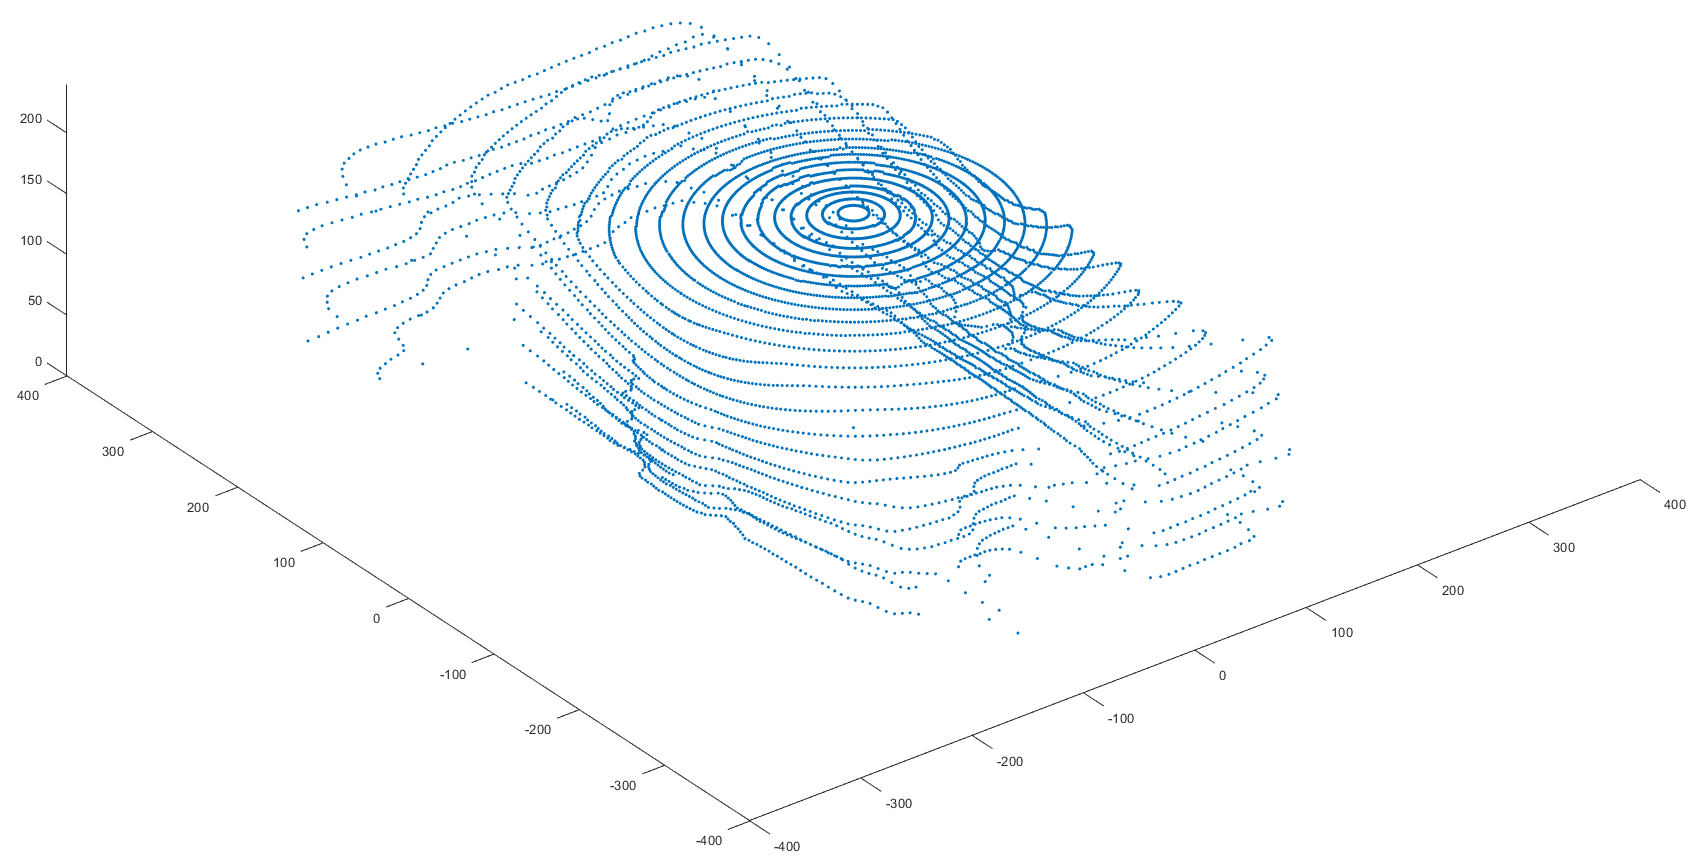
\includegraphics[width=0.9\textwidth]{images/Validierung/Aufloesungen/niedrig.png}
	\caption{Niedrige Auflösung}
	\label{niedrig}
\end{figure}


Bei der mittleren Auflösung werden etwa 16 mal so viele Bildpunkte aufgenommen wie bei der Messung mit geringer Auflösung. Die vertikale Schrittweite wird im Verglich zur ersten Messung halbiert, die horizontale beträgt mit 0,15 Grad ein Achtel der ursprünglichen Schrittweite. 

Die horizontalen Punkte verschmelzen zu einer Linie. Dies ist ein Zeichen dafür, dass die horizontale Auflösung von 0,15 Grad für den Testraum ausreichend ist. Durch die geringere vertikale Schrittweite erhält man doppelt so viele Messebenen. Dadurch werden Details wie beispielsweise Türrahmen, Lampen und weitere Gegenstände besser erkennbar. 


\begin{figure}[H]
	\centering
	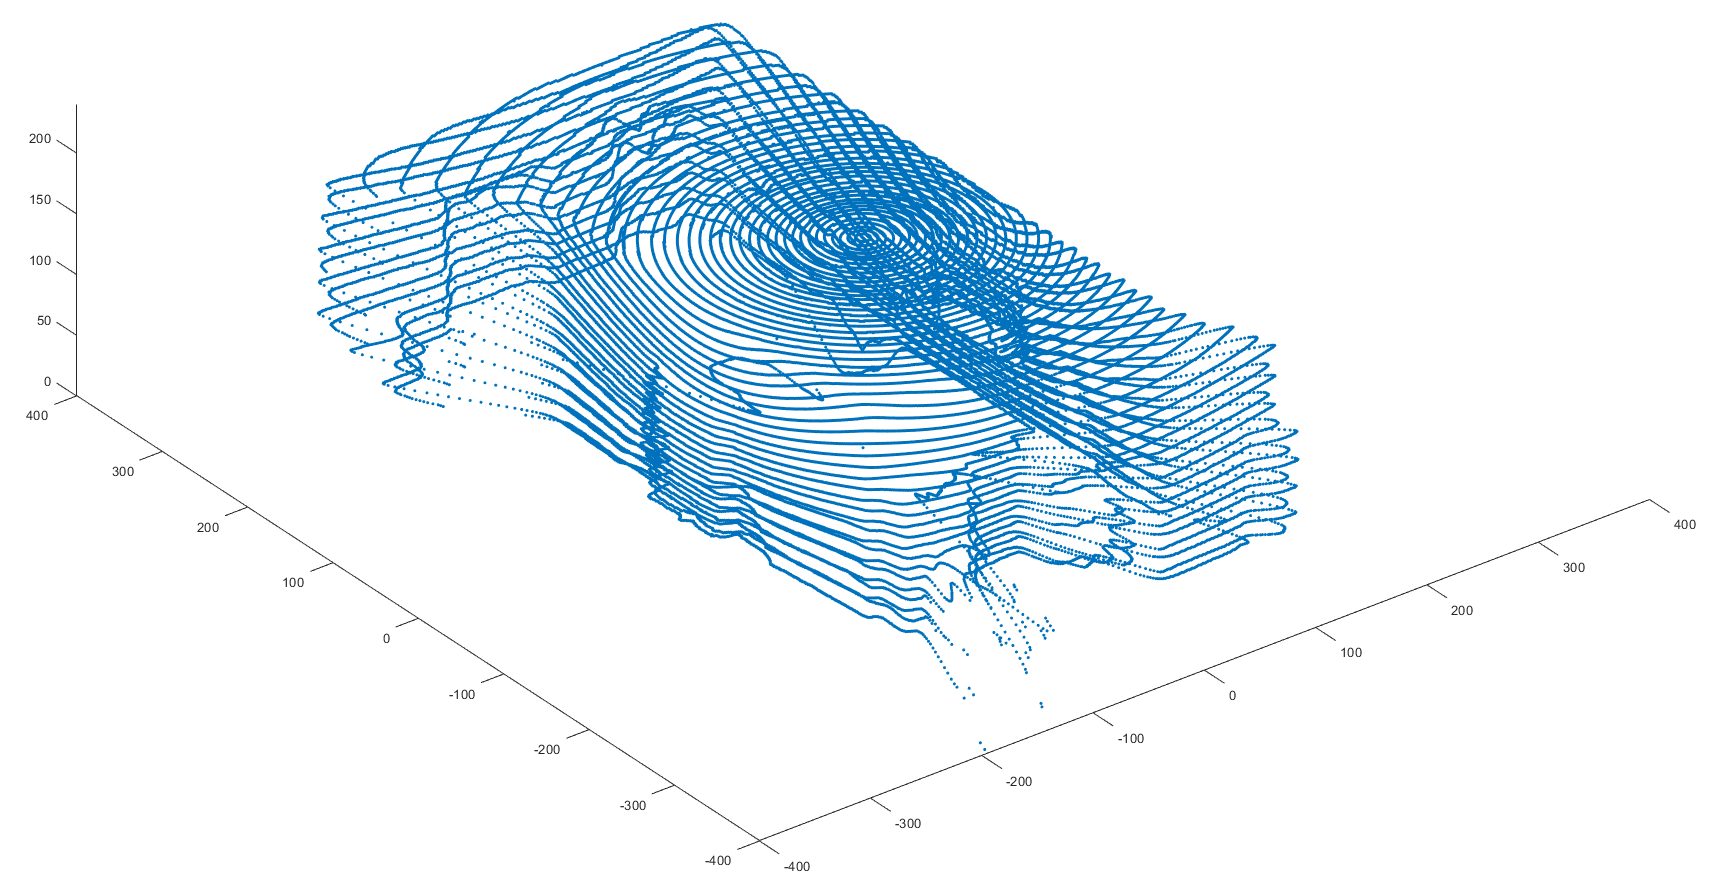
\includegraphics[width=0.9\textwidth]{images/Validierung/Aufloesungen/mittel.png}
	\caption{Mittlere Auflösung}
	\label{mittel}
\end{figure}

Wie die Messung mit mittlerer Auflösung bereits gezeigt hat, reicht eine horizontale Schrittweite von 0,15 Grad bei der Größe des Testraums aus. Für den Test mit hoher Auflösung wird daher nur noch die vertikale Schrittweite halbiert. Dadurch verdoppelt sich die Anzahl der Bildpunkte. Die Messung benötigt jedoch ungefähr doppelt so lange.

Das Ergebnis ist eine 3D-Aufnahme, bei der sowohl horizontale als auch vertikale Auflösung gut ausreicht, um Details erkennen zu können.

\begin{figure}[H]
	\centering
	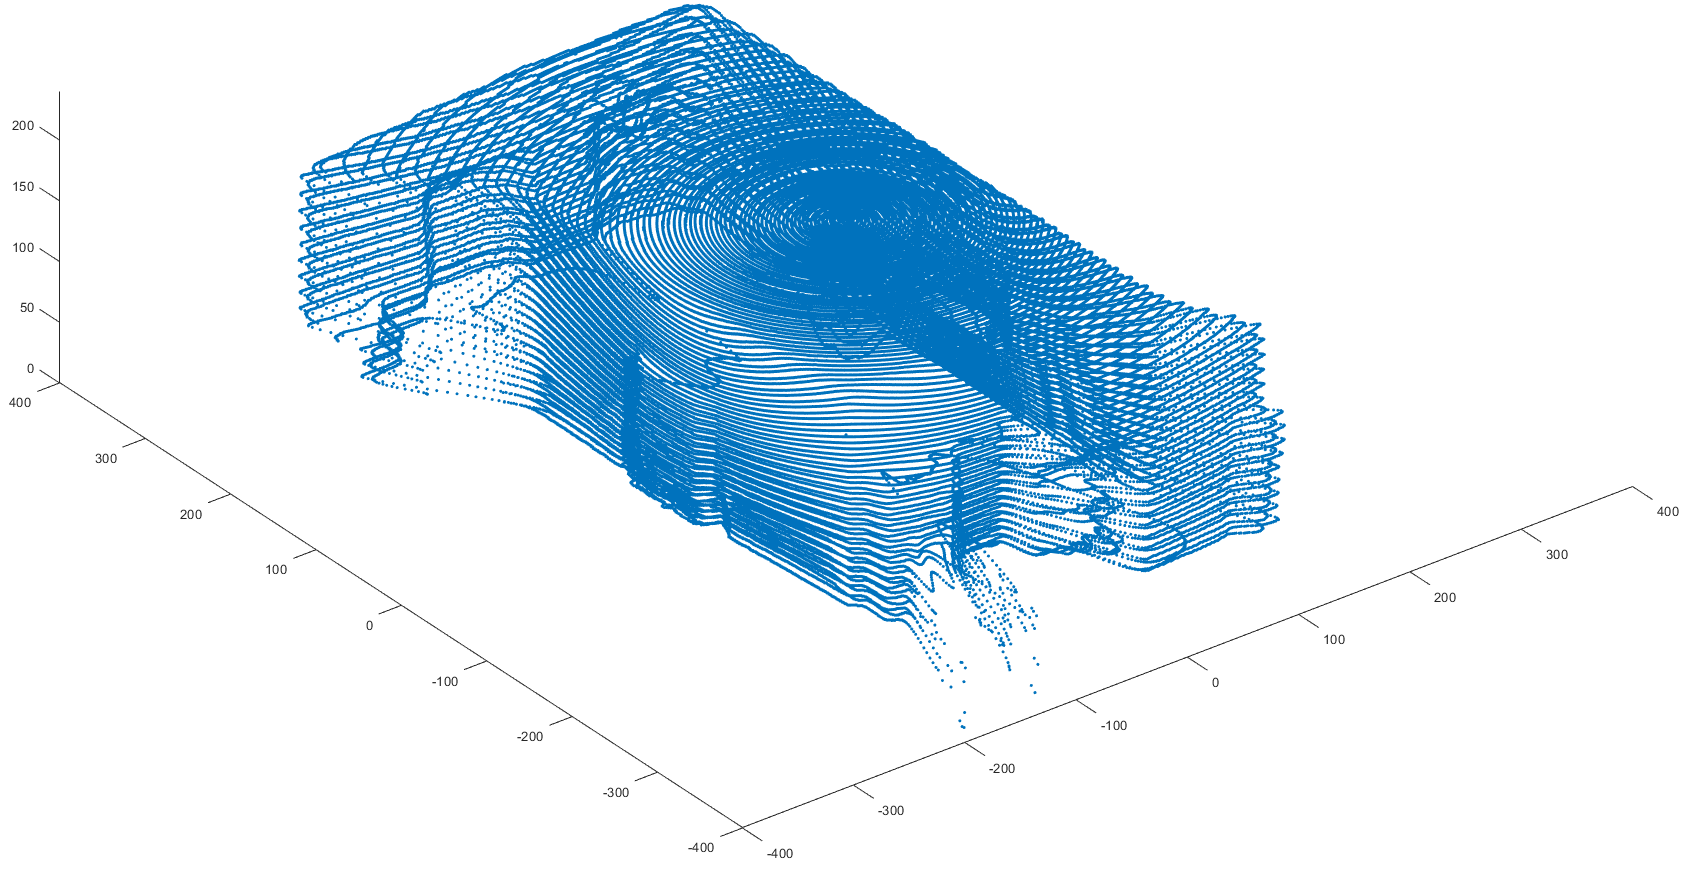
\includegraphics[width=0.9\textwidth]{images/Validierung/Aufloesungen/hoch.png}
	\caption{Hohe Auflösung}
	\label{hoch}
\end{figure}



% Bilder von abständen +auflösung, kann das stimmen?
%näher dran
\begin{figure}[htb]
	\centering
	\begin{minipage}[t]{0.45\linewidth}
		\centering
		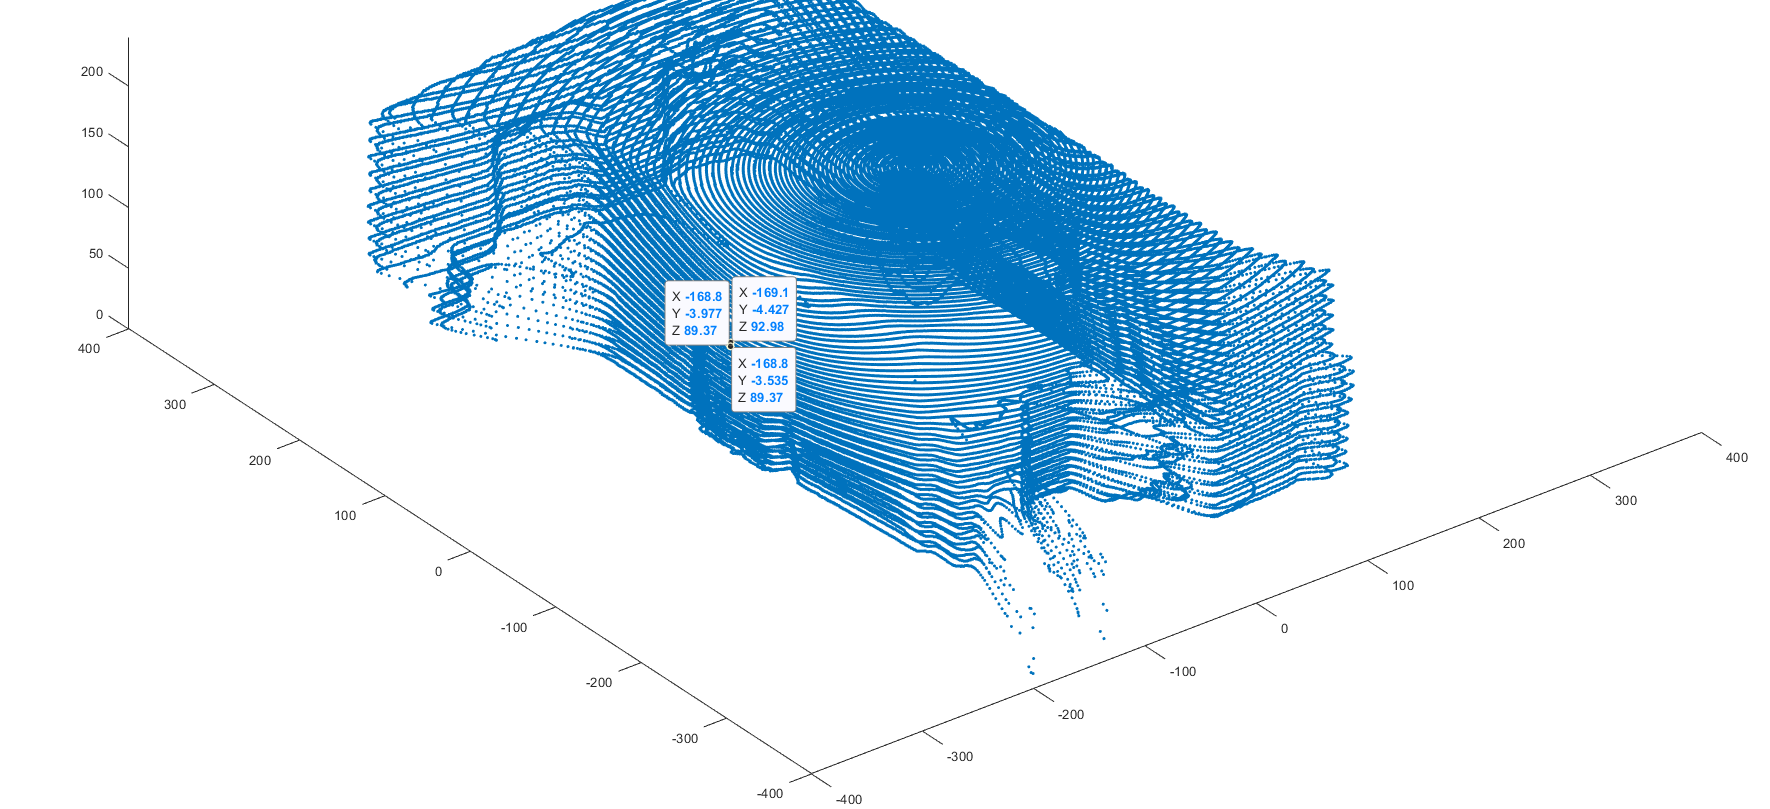
\includegraphics[width=1.2\linewidth]{images/Validierung/Aufloesungen/3Messwerte_Ansicht.png}
		\caption{Vogelperspektive niedrige Auflösung}
		\label{vogasdasdel niedrigeAuflösung}
	\end{minipage}
	\hfill
	\begin{minipage}[t]{0.45\linewidth}
		\centering
		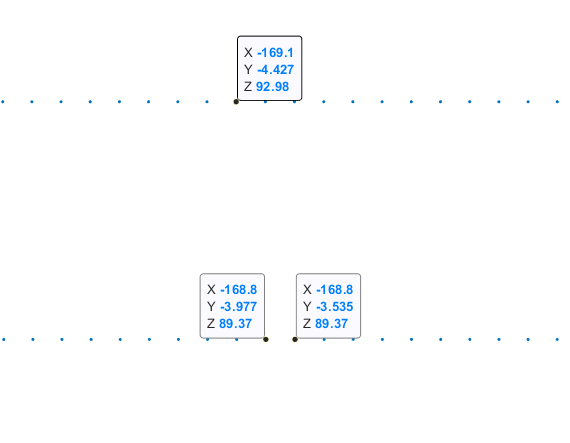
\includegraphics[width=1.2\linewidth]{images/Validierung/Aufloesungen/3Label.png}
		\caption{Vogelperspektive hohe Auflösung}
		\label{vogel hoheAsadasduflösung}
	\end{minipage}
\end{figure}

%weiter weg

\begin{figure}[htb]
	\centering
	\begin{minipage}[t]{0.45\linewidth}
		\centering
		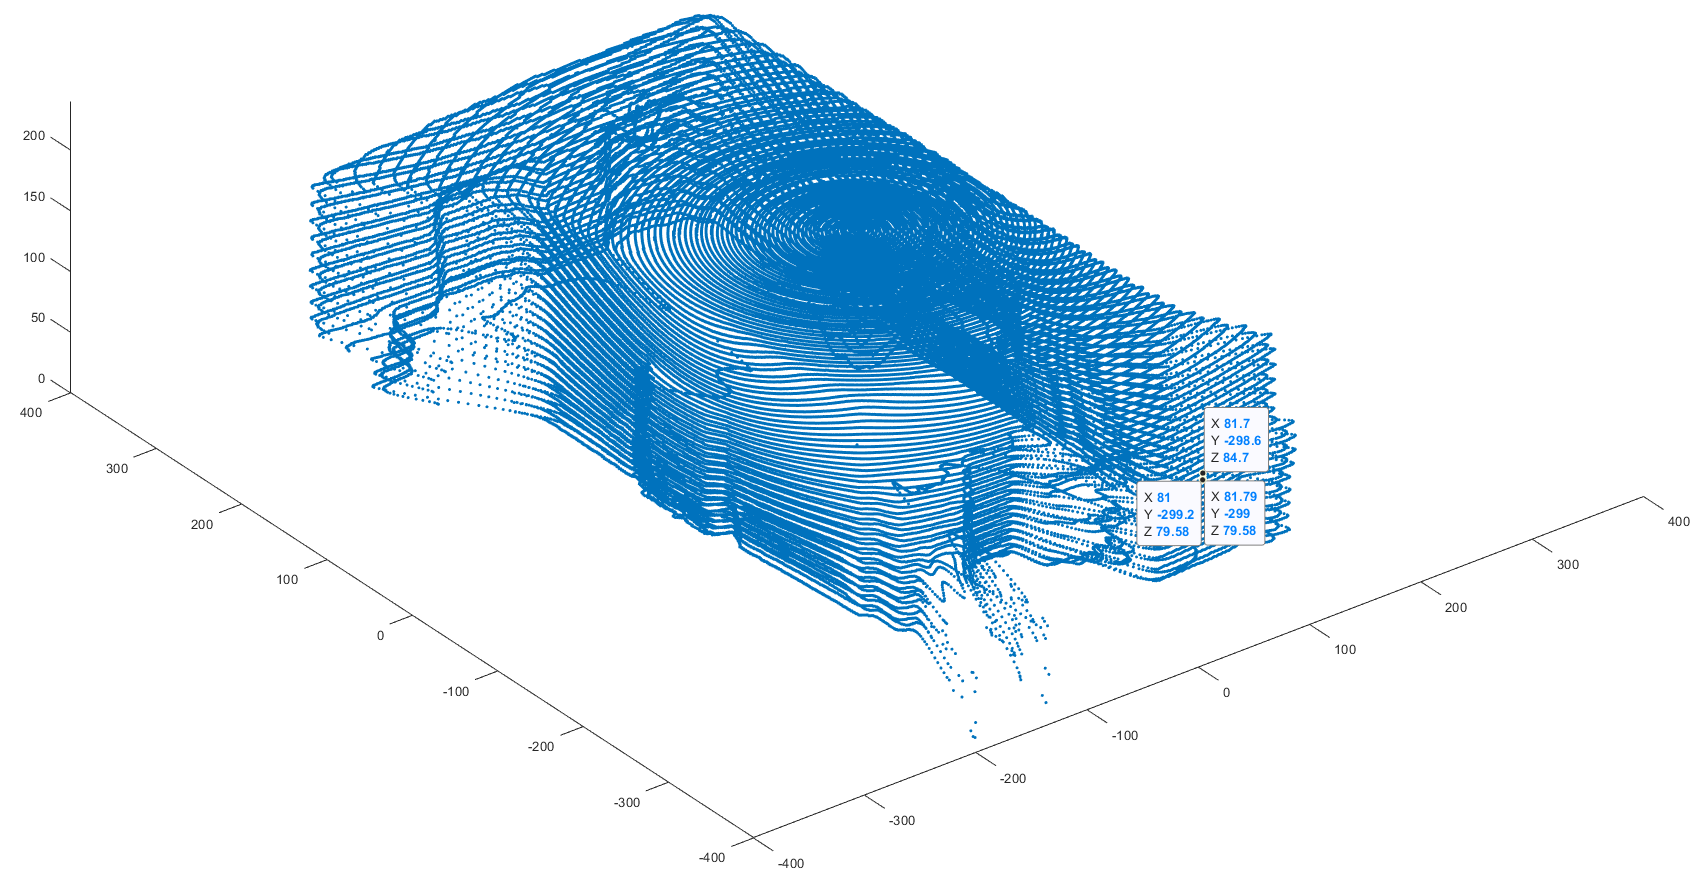
\includegraphics[width=1.2\linewidth]{images/Validierung/Aufloesungen/3Messwerte_Wand.png}
		\caption{Vogelperspektive niedrige Auflösung}
		\label{vogel niedriasdasgeAuflösung}
	\end{minipage}
	\hfill
	\begin{minipage}[t]{0.45\linewidth}
		\centering
		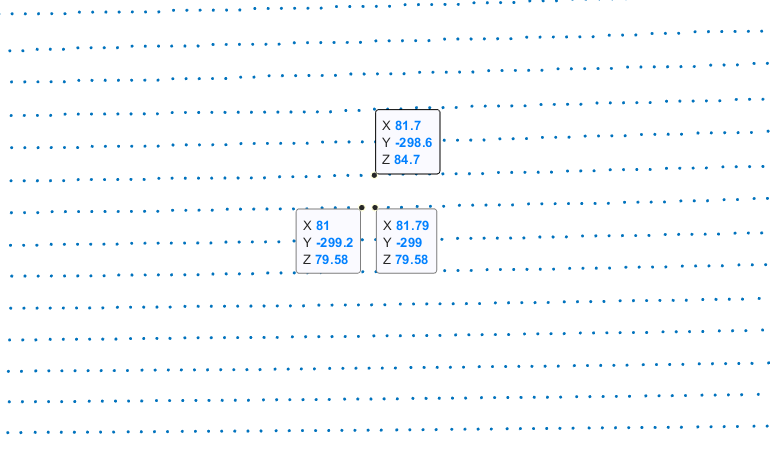
\includegraphics[width=1.2\linewidth]{images/Validierung/Aufloesungen/Wand_3Messungen.png}
		\caption{Vogelperspektive hohe Auflösung}
		\label{vogel hohasdeAuflösung}
	\end{minipage}
\end{figure}


Weiter werden die erstellten Grundrisse mit niedriger, mittlere und hoher Auflösung mit dem tatsächlichen Grundriss verglichen.

Der Vergleich zeigt, dass die Maße immer bis auch geringe Abweichungen mit dem tatsächlichen Grundriss übereinstimmten. Dabei macht die Auflösung keinen Unterschied. 

Deutlich erkennbar ist jedoch, wie in Abbildung \ref{vogel niedrigeAuflösung} zu sehen ist, dass bei niedriger Auflösung Details wie Türrahmen verschwimmen. Zudem sind die einzelnen Linienebenen leicht zueinander verschoben und nicht eindeutig zuordenbar.
Im Vergleich dazu sind bei der hohen Auslösung (Abbildung \ref{vogel hoheAuflösung}) klare Grundrisslinien erkennbar.

\begin{figure}[htb]
	\centering
	\begin{minipage}[t]{0.45\linewidth}
		\centering
		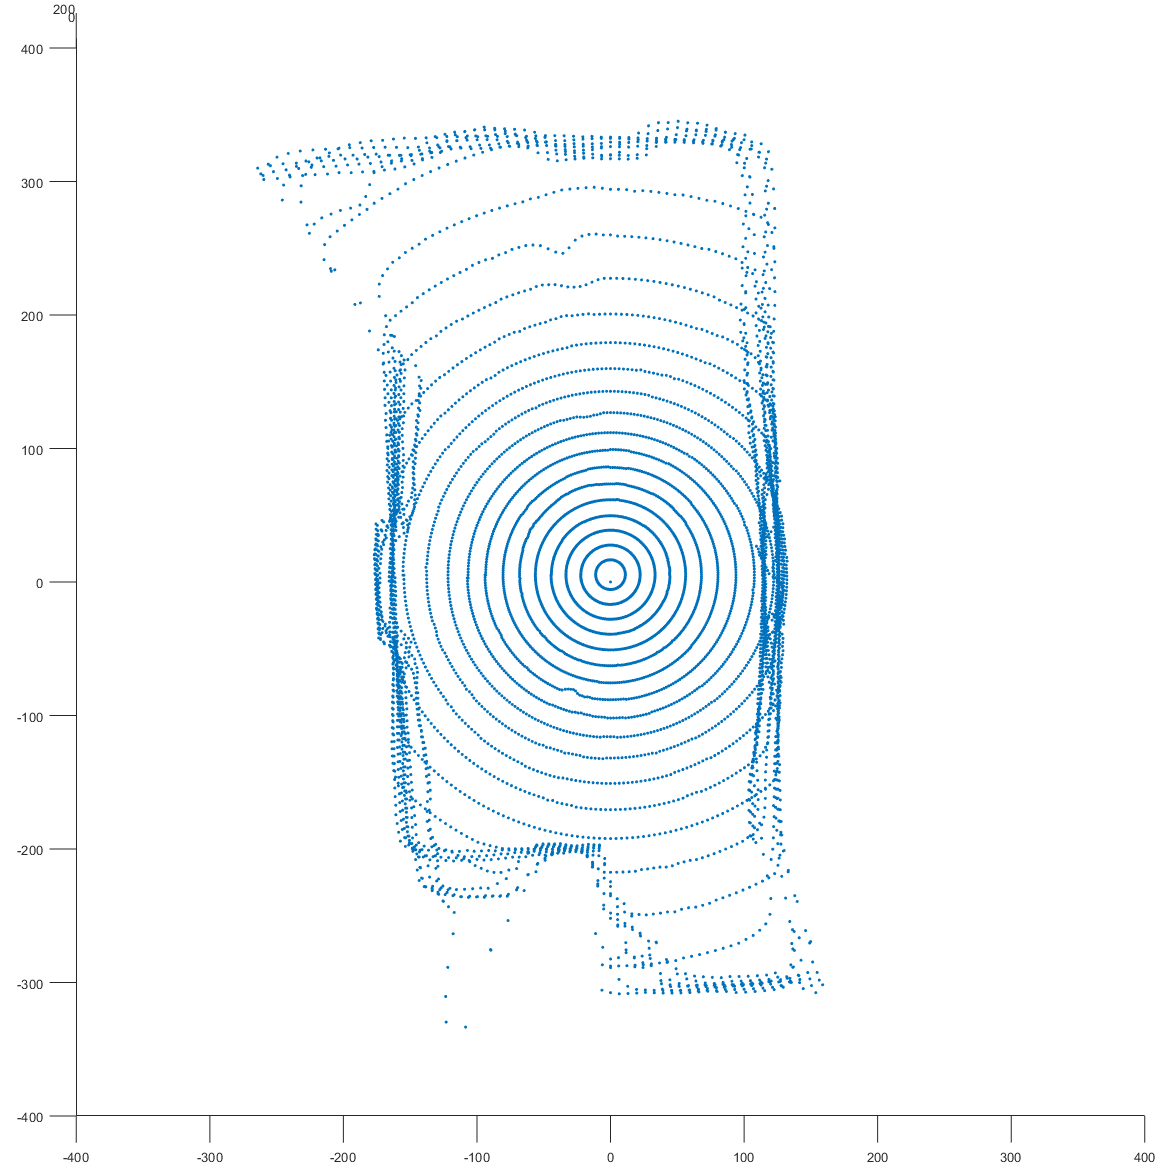
\includegraphics[width=1.2\linewidth]{images/Validierung/Aufloesungen/niedrig_vogel.png}
		\caption{Vogelperspektive niedrige Auflösung}
		\label{vogel niedrigeAuflösung}
	\end{minipage}
	\hfill
	\begin{minipage}[t]{0.45\linewidth}
		\centering
		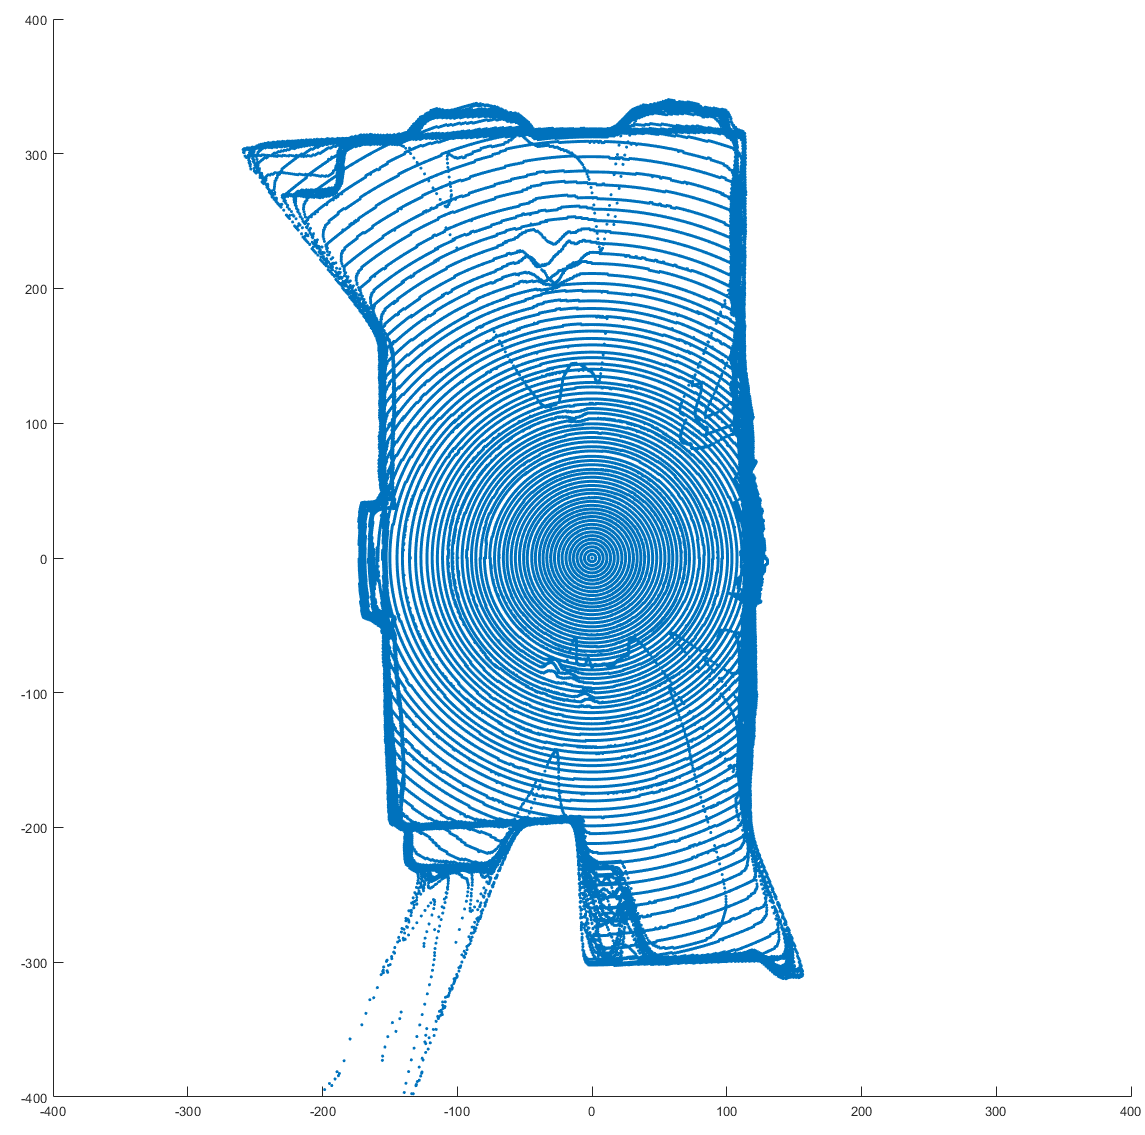
\includegraphics[width=1.2\linewidth]{images/Validierung/Aufloesungen/hoch_vogel.png}
		\caption{Vogelperspektive hohe Auflösung}
		\label{vogel hoheAuflösung}
	\end{minipage}
\end{figure}


Im Großen und Ganzen lässt sich sagen, dass je nach Anforderung an das System die Parameter dementsprechend eingestellt werden müssen. Möchte man nur einen groben Überblick über den Raum, reicht ein schneller Scan mit niedriger Auflösung vollkommen aus. Möchte man hingegen eine detailreiche Darstellung, bei der man auch Details virtuell vermessen kann, wird eine hohe Auflösung benötigt. Dafür dauert solch eine Messung im Vergleich zur schnellen Messung recht lange.
Man sollte somit immer einen Kompromiss zwischen benötigter Auflösung und der Zeit für die Messung finden.



\section{Vergleich der Sensoren}

Nachdem sowohl die Mechanik als auch der erste Lidar Sensor getestet und validiert wurden, soll ein kostengünstigerer Sensor getestet werden. Dazu werden zwei Aufnahmen mit den gleichen Einstellungen aber verschiedenen Sensoren aufgenommen. Die erste Messung wird mit dem Sensor "TF MINI" gemacht. Als zweiter Sensor wird der Sensor "VL53L1X" verwendet.

 

\begin{figure}[H]
	\centering
	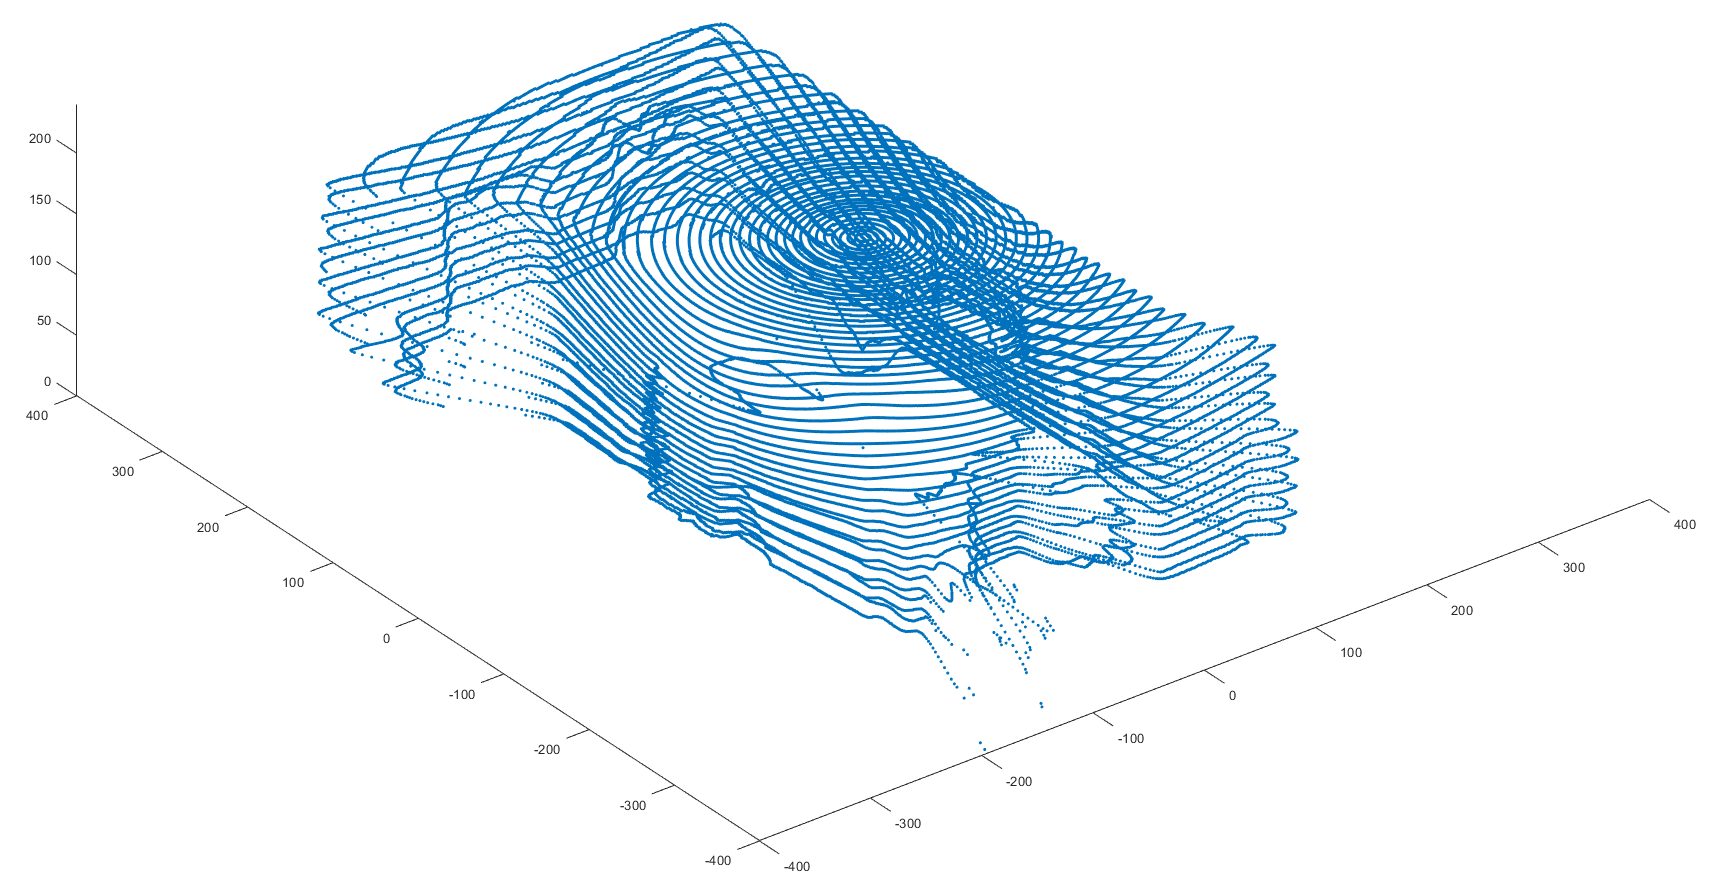
\includegraphics[width=0.9\textwidth]{images/Validierung/Aufloesungen/mittel.png}
	\caption{Sensorvergleich: TF MINI}
	\label{hoch}
\end{figure}



\begin{figure}[H]
	\centering
	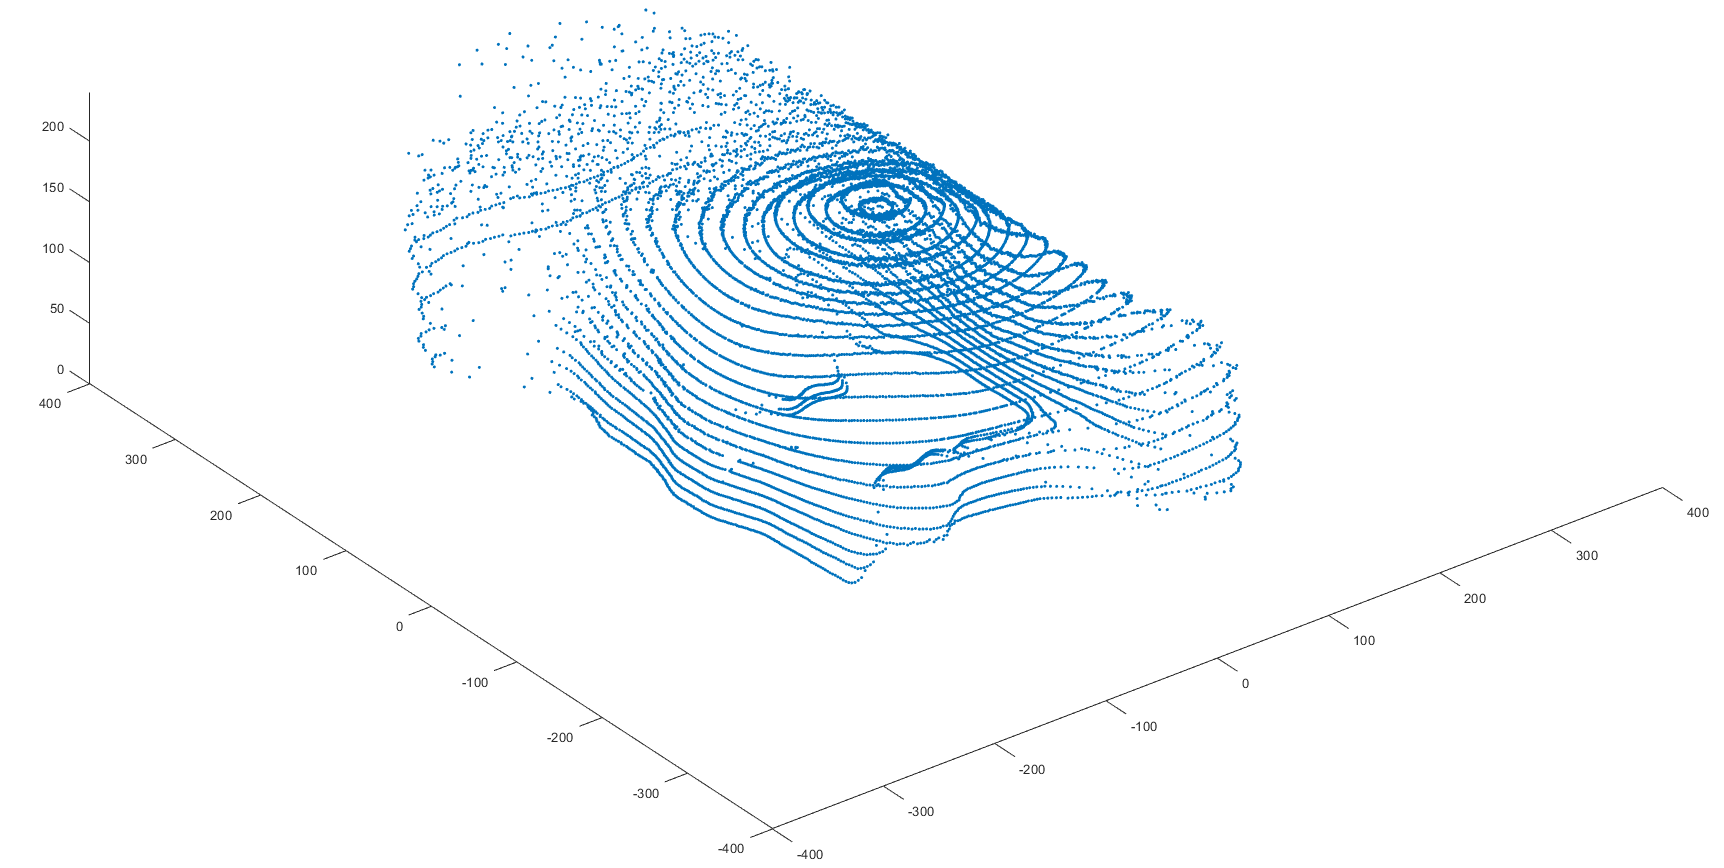
\includegraphics[width=0.9\textwidth]{images/Validierung/VL53.png}
	\caption{Sensorvergleich: VL53L1X}
	\label{vlx}
\end{figure}

Bei den Aufnahmen der Sensoren sind trotz selber Einstellungen sehr deutliche Unterschiede erkennbar. Während die Aufnahme mit dem "TF MINI" Sensor sehr deutliche Konturen erkennen lässt, verschwimmen diese bei dem zweiten Sensor. Es ist Auffallend, dass vor allem weiter entfernte Punkte nicht sauber aufgezeichnet werden können. So ist die Wand links oben beispielsweise nicht als solche zu erkenne. Die Punkte streuen zu sehr. Dies liegt vermutlich an der maximalen messbaren Distanz von 4 Metern bei optimalen Umgebungsbedingungen. Diese Bedingungen und Abhängigkeiten sind in Kapitel \ref{VL53L1X} genauer aufgeführt. Es kann davon ausgegangen werden, dass die Bedingungen bei der Messung nicht optimal waren und dewegen die maximal messbare Distanz kleiner war, als die Distaz, in der sich die Wand von dem Sensor befunden hat. 

Die folgenden beiden Abbildungen zeigen noch die jeweilige Vogelperspektive. \\



\begin{figure}[htb]
	\centering
	\begin{minipage}[t]{0.45\linewidth}
		\centering
		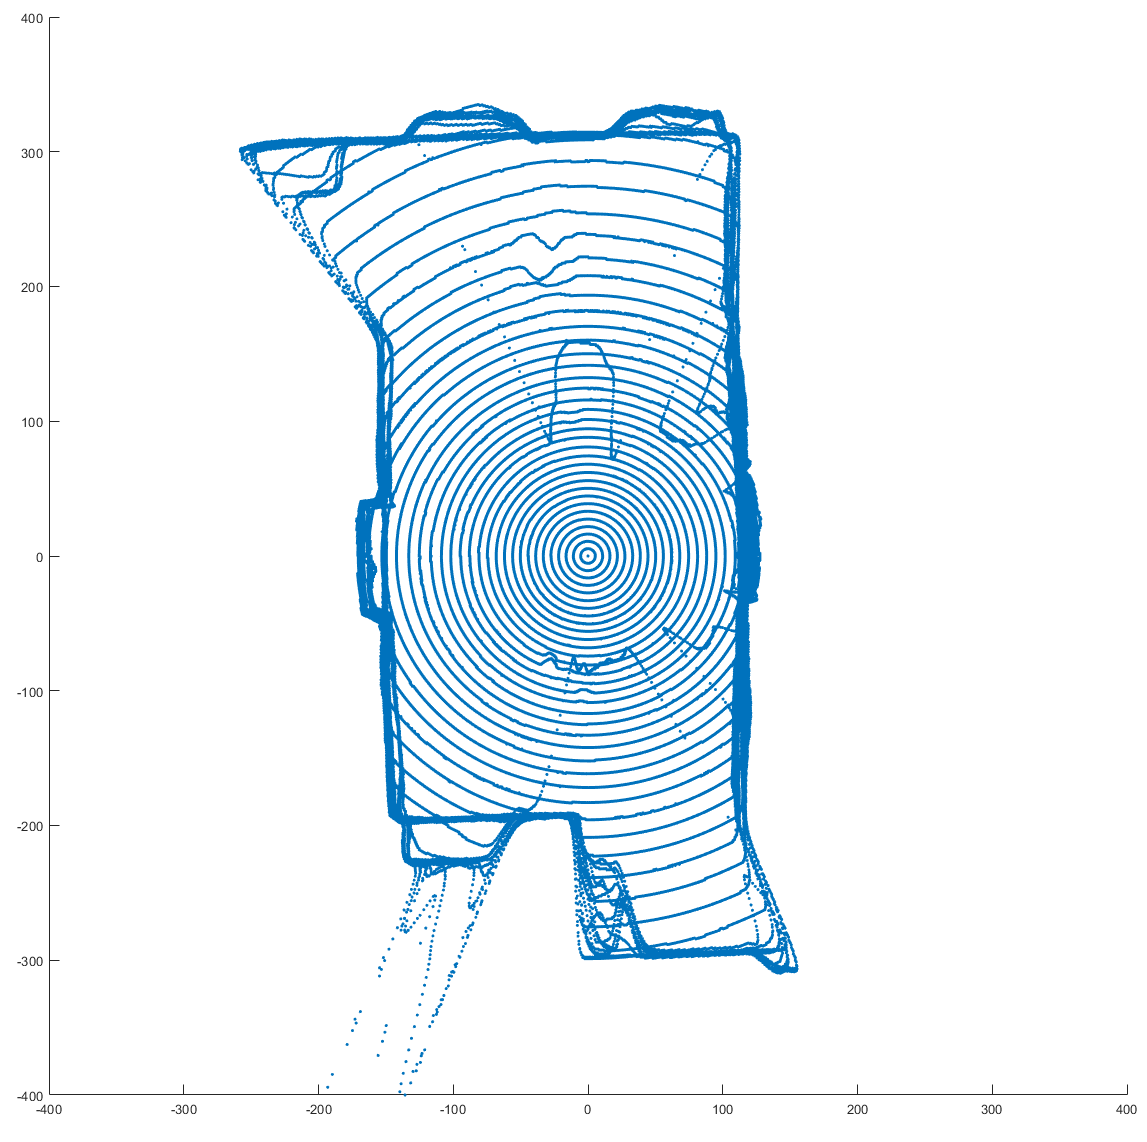
\includegraphics[width=1.2\linewidth]{images/Validierung/Aufloesungen/mittel_vogel.png}
		\caption{TF MINI - Vogelperspektive}
	\end{minipage}
	\hfill
	\begin{minipage}[t]{0.45\linewidth}
		\centering
		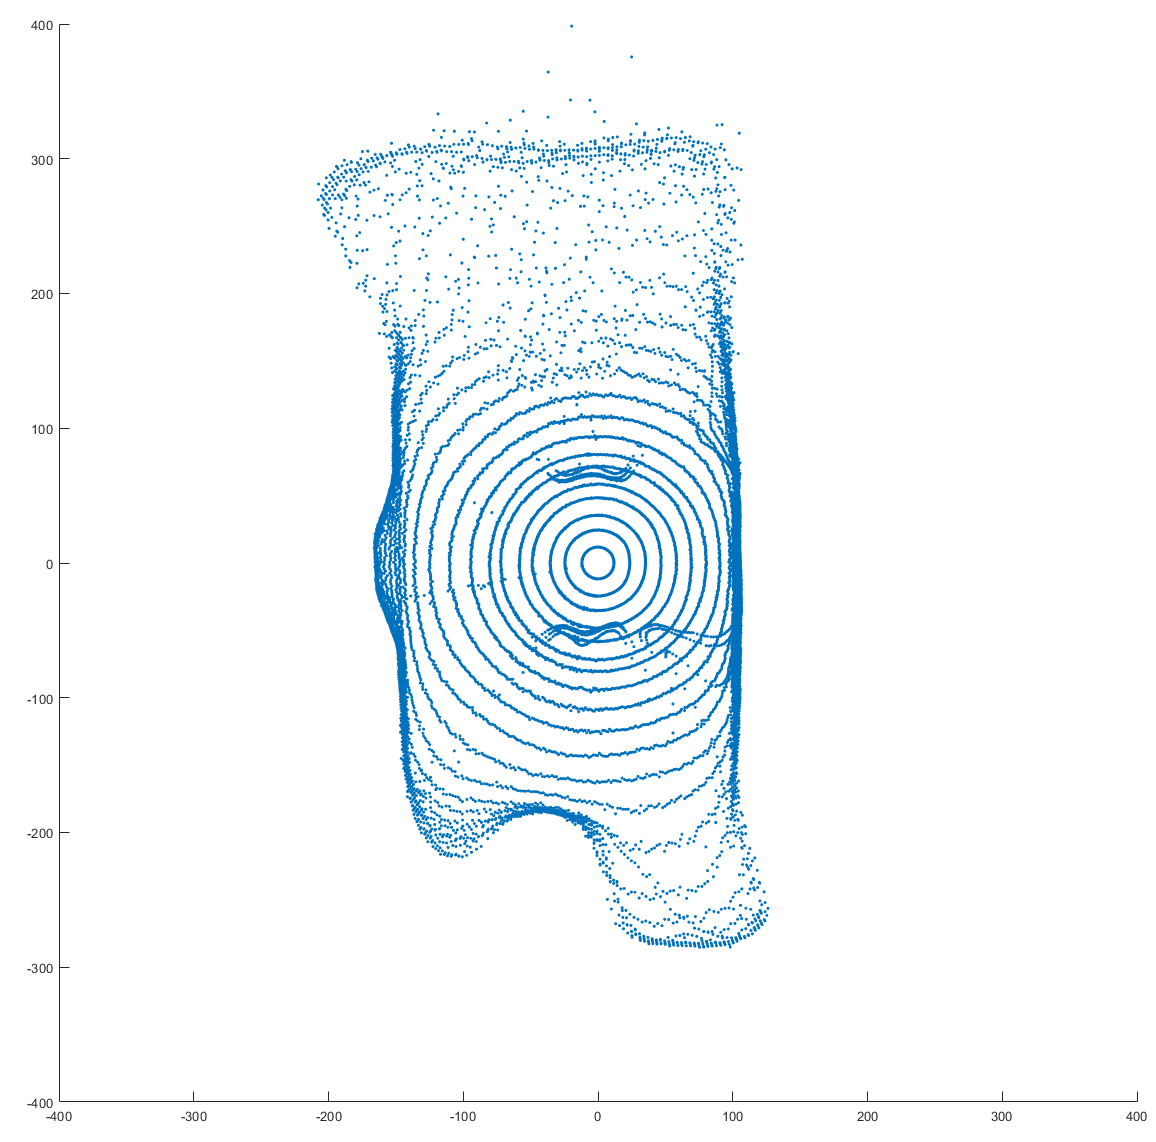
\includegraphics[width=1.2\linewidth]{images/Validierung/VL53_vogel.png}
		\caption{Sensor VL53L1X - Vogelperspektive}
	\end{minipage}
\end{figure}


Auch bei dieser Abbildung ist zu erkennen, dass der erste Sensor viel deutlichere Konturen abbildet und die Messungenauigkeit deutlich geringer ist. Sowohl nahe als auch weiter entfernte Wände werden zuverlässig erkannt. Beim zweiten Sensor wird wieder deutlich, dass alle Punkte, die etwas weiter vom Messpunkt entfernt sind, nur sehr ungenau oder gar nicht aufgenommen werden. 

Der Vergleich zeigt, dass der kostengünstigere Sensor "VL53L1X" unbrauchbar für das System ist. Die maximal messbare Distanz ist mit 4 Metern nur knapp über der Anforderung. Diese Distanz ist jedoch nur bei optimalen Umgebungsbedingungen realisierbar. Weichen diese Bedinungen beispielsweise durch schlecht Reflektierende Wände oder Umgebungslicht ab, sinkt die maximal messbare Distanz und die Messungenauigkeit steigt.  Dadurch entstehende fehlerhafte Abbildungen wie beispielsweise Abbildung \ref*{vlx}. Um dies zu verhindern, müssten die Umgebungsbedingungen dauerhaft angepasst und überwacht werden, was im Konflikt zu der Anforderung der Benutzerfreundlichkeit steht.\\

Der etwas teurere Sensor "TF MINI" hat in diesem Vergleich klar überzeugt. Unabhängig von Umgebungslicht, Reflexionseigenschaften der Wand und weiterer Parameter werden die Messwerte zuverlässig aufgenommen. 

\todo{Ausführlicher?}






